% !TeX encoding = UTF-8

\documentclass{protokol}

\usepackage{pdfpages}
\usepackage{tikz}
\usetikzlibrary{calc}
\usetikzlibrary{arrows}

%====== Units =====
\usepackage{siunitx}
\sisetup{inter-unit-product =\ensuremath{\cdot}}
\sisetup{group-digits = integer}
\sisetup{output-decimal-marker = {,}}
\sisetup{exponent-product = \ensuremath{\cdot}}
\sisetup{separate-uncertainty}
\sisetup{tight-spacing = false}
%\sisetup{scientific-notation = true}
%\sisetup{round-mode=places,round-precision=4}
%\sisetup{evaluate-expression}


%====== Grafy =====
\usepackage{pgfplots}
\pgfplotsset{width=0.8\linewidth, compat=1.17}
\def\plotcscale{0.8}
\usepackage{pgfplotstable}
\usepackage[figurename=Obr.]{caption} % figure caption rename

%====== Rovnice align block ======
\usepackage{amsmath}
\setlength{\jot}{10pt} % rozestup mezi řádky

\graphicspath{ {./img/} }

%====== Vyplňte údaje ======
\jmeno{Jakub Charvot}
\kod{240844}
\rocnik{3.}
\obor{MET}
\skupina{MET/2}
\spolupracoval{--}

\merenodne{19.02.\ 2024}
\odevzdanodne{25.02.\ 2024}
\nazev{Extrakce parametrů tranzistorů MOSFET ze SPICE modelu }
\cislo{1} %měřené úlohy

\predmet{Návrh analogových integrovaných obvodů}
\ustav{Ústav mikroelektroniky}
\skola{FEKT VUT v~Brně}

\def\para{x+0}
\def\parb{\para-80}


%citace 
\usepackage[backend=biber, style=iso-numeric, sortlocale=cs_CZ, autolang=other, language=czech]{biblatex}
\addbibresource{bibliography.bib}
\DeclareFieldFormat{labelnumberwidth}{\mkbibbrackets{#1}}
% hyperlinky
\usepackage[colorlinks]{hyperref}

% odstavce
\usepackage{parskip}

% Bloky kódu
\usepackage{xcolor}

%New colors defined below
\definecolor{codegreen}{rgb}{0,0.6,0}
\definecolor{codegray}{rgb}{0.5,0.5,0.5}
\definecolor{codepurple}{rgb}{0.58,0,0.82}
\definecolor{backcolour}{rgb}{0.95,0.95,0.92}

\usepackage{listings}
\lstdefinestyle{mystyle}{
  backgroundcolor=\color{backcolour}, commentstyle=\color{codegreen},
  keywordstyle=\color{magenta},
  numberstyle=\tiny\color{codegray},
  stringstyle=\color{codepurple},
  basicstyle=\ttfamily\footnotesize,
  breakatwhitespace=false,         
  breaklines=true,                 
  captionpos=b,                    
  keepspaces=true,                 
  numbers=left,                    
  numbersep=5pt,                  
  showspaces=false,                
  showstringspaces=false,
  showtabs=false,                  
  tabsize=2
}
\lstset{
	inputencoding=utf8,
	extendedchars=true,
	literate={á}{{\'a}}1 {č}{{\v{c}}}1 {ď}{{\v{d}}}1 {é}{{\'e}}1 {ě}{{\v{e}}}1 
           {í}{{\'i}}1 {ň}{{\v{n}}}1 {ó}{{\'o}}1 {ř}{{\v{r}}}1 {š}{{\v{s}}}1 
           {ť}{{\v{t}}}1 {ú}{{\'u}}1 {ů}{{\r{u}}}1 {ý}{{\'y}}1 {ž}{{\v{z}}}1 
           {Á}{{\'A}}1 {Č}{{\v{C}}}1 {Ď}{{\v{D}}}1 {É}{{\'E}}1 {Ě}{{\v{E}}}1 
           {Í}{{\'I}}1 {Ň}{{\v{N}}}1 {Ó}{{\'O}}1 {Ř}{{\v{R}}}1 {Š}{{\v{S}}}1 
           {Ť}{{\v{T}}}1 {Ú}{{\'U}}1 {Ů}{{\r{U}}}1 {Ý}{{\'Y}}1 {Ž}{{\v{Z}}}1,
	style=mystyle
	}

% Číslování
\pagenumbering{arabic}

% =========================================
% =============== DOKUMENT ================
% =========================================
\begin{document}
	%====== Vygenerování tabulky ======
	\maketitle

\section{Vypracování}
  Pro provedení všech simulací jsem použil dvě zapojení, jedno pro tranzistor typu NMOS (viz Obr.~\ref{fig:img-nmos-png}), druhé pak pro typ PMOS (Obr.~\ref{fig:img-pmos-png}). Napájecí uzly jsem definoval pro obě zapojení stejně, jako je vidět na třetím schématu na Obr.~\ref{fig:img-power-png}.

  SPICE kód potřebný pro simulace jsem rozdělil do několika bloků (viz Obr.~\ref{fig:img-spice-png}) a vždy přepínal mezi komentářem a spustitelným kódem. Díky tomu jsem omezil duplicitní kód a mohl využít obě schémata jednoduše pro všechny tři simulace, vždy s výběrem vhodné kombinace bloků. Bohužel s tímto konceptem možná drobně klesá přehlednost.

  \begin{figure}[h!]
    \centering
    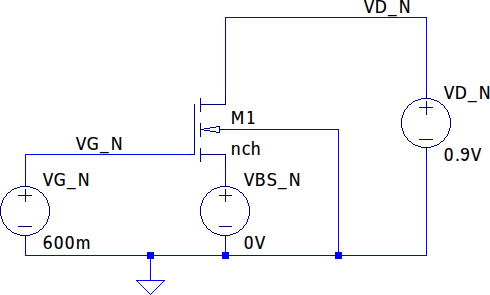
\includegraphics[scale=1]{img/nmos.png}
    \caption{Zapojení s tranzistorem NMOS.}
    \label{fig:img-nmos-png}
  \end{figure}

  \begin{figure}[h!]
    \centering
    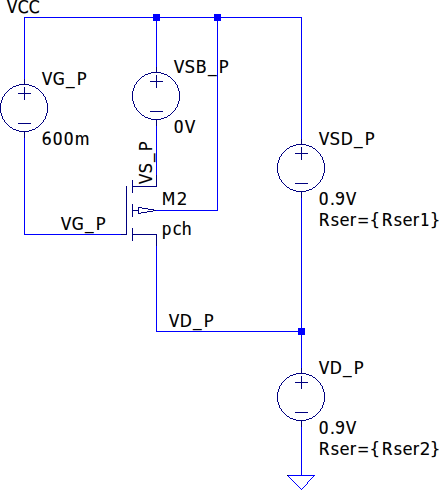
\includegraphics[scale=1]{img/pmos.png}
    \caption{Zapojení s tranzistorem PMOS.}
    \label{fig:img-pmos-png}
  \end{figure}

  \begin{figure}[h!]
    \centering
    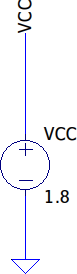
\includegraphics[scale=1]{img/power.png}
    \caption{Definice uzlů napájení pro zbylé obvody.}
    \label{fig:img-power-png}
  \end{figure}

  \begin{figure}[h!]
    \centering
    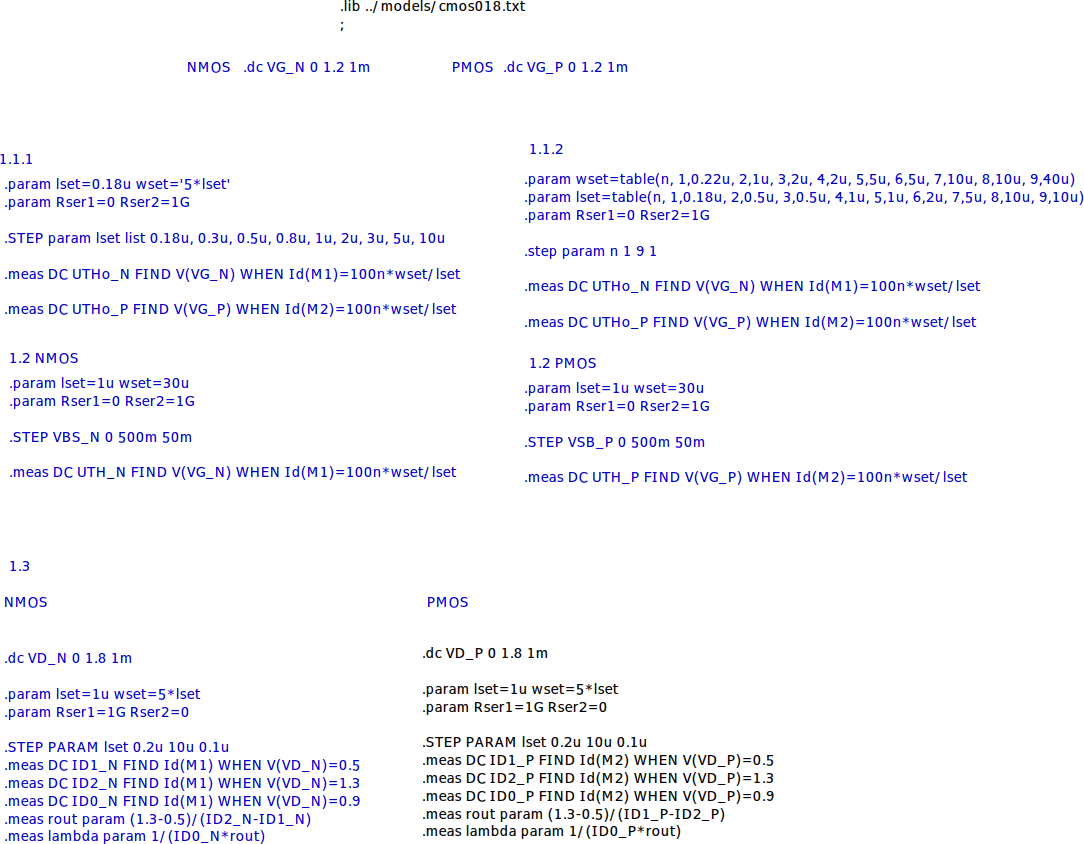
\includegraphics[width=\textwidth]{img/spice.png}
    \caption{Všechny použité bloky SPICE kódy.}
    \label{fig:img-spice-png}
  \end{figure}


  \clearpage
\subsection{Výpočty }
Nejprve vypočítám rozměry pro tranzistor \(M_{N1} \):
\[
    \frac{W_{N1} }{L}=\frac{2\cdot I_{D}}{KP_{N}\cdot (U_{GS} -U_{TH})^2 } 
\]
\[
    \frac{W_{N1} }{L}=\frac{2\cdot \num{20e-6}}{\num{220e-6}\cdot (\num{0.2})^2 } 
\]

\[
    \frac{W_{N1} }{L}\doteq \num[round-mode=places,round-precision=2]{4.545454545454545} 
\]
Délku \(L\) zvolíme opět \qty{2}{\micro\meter}, tedy \(W_{N1}= \qty{9.09}{\micro\meter}\). Pro tranzistor \(M_{N2} \) zvolíme stejné rozměry.

Pro tranzistory \(M_{P1} \) a \(M_{P2} \) vypočteme rozměry obdobným způsobem:

\[
    \frac{W_{P12} }{L}=\frac{2\cdot I_{D}}{KP_{P}\cdot (U_{GS} -U_{TH})^2 } 
\]
\[
    \frac{W_{P12} }{L}=\frac{2\cdot \num{20e-6}}{\num{60e-6}\cdot (\num{0.2})^2 } 
\]

\[
    \frac{W_{P12} }{L}\doteq \num[round-mode=places,round-precision=2]{16.666666666666664}
\]

Pro stejnou délku \(L\) pak vychází \(W_{P12}=\qty{33.33}{\micro\meter} \).













\subsection{Minula uloha}

\[
    \frac{W_{1} }{L_{1} }\doteq \num[round-mode=places,round-precision=2]{5.681818181818182} 
\]
Pro oba tranzistory zvolíme stejnou délku kanálu \(L_{1}=L_{2} = \qty{0.2}{\micro\meter}\), tedy \(W_{1} =\qty[round-mode=places,round-precision=2]{1,136363636363636}{\micro\meter}\). Druhý tranzistor má dosáhnout dvakrát vyššího proudu, takže zvolíme \(W_{2} =\qty{2.28}{\micro\meter}\)  

\[
    R_1=\frac{U_R}{I_{M 1}}=\frac{U_{C C}-U_{G S 1}}{I_{M 1}}=\frac{U_{C C}-\left(U_{T H 0,1}+U_{O V, 1}\right)}{I_{M 1}}
\]
\[
    R_1=\frac{\num{1.8}-\left(\num{368,024e-3}+\num{0.2}\right)}{\num{25e-6}}
\]
\[
    R_{1} \doteq \qty{49,28}{\kilo\ohm}
\]


\[
    r_{O U T}=\frac{1}{\lambda \cdot I_{M 2}}
\]

\[
    r_{O U T}=\frac{1}{\num[round-mode=places,round-precision=3]{0,0437895} \cdot \num{50e-6}}
\]
\[
    r_{O U T}=\qty[round-mode=places,round-precision=3]{454,5454545454545}{\kilo\ohm}
\]



\subsubsection{Kaskodové}
Pro vstupní větev je stanoven proud \qty{50}{\micro\ampere}, výpočet rozměrů je proveden obdovným způsobem jako v minulém přkladu:
\[
    \frac{W_3}{L_3}=\frac{2\cdot I_{D3}}{KP_{P}\cdot (U_{GS} -U_{TH})^2 } 
\]
\[
    \frac{W_3}{L_3}=\frac{2\cdot \num{50e-6}}{\num{60e-6} \cdot (\num{0.2})^2 } 
\]
\[
    \frac{W_3}{L_3}=\num{41,67}
\]

Pro nastavení proudu slouží rezistor R2. Jeho hodnota je stanovena na základě úbytku napětí na rezistoru.
% U_bs pro M3 je U_GS1 coz je U_th0 + U_ov
% z tabulky pak odecitam radek pro nejvyssi U_bs, coz je porad mene...
% zaokrouhleno nahoru 600m
\begin{align*}
    U_{R 2}=&U_{C C}-U_{G S 1}-U_{G S 3} \\
           =&U_{C C}-U_{T H 0,1}- U_{O V 1}-U_{T H, 3}-U_{O V 3} \\
           =&U_{C C}-U_{T H 0,1}-U_{T H, 3}-2 \cdot U_{O V 1,3} \\
           =&\num{1.8}-\num{0.4433}-\num{0.6}-2 \cdot \num{0.2} \\
           =&\qty{0.3567}{\volt}
\end{align*}

\begin{align*}
    R_{2} =& \frac{U_{R1}}{I_{M1} } \\
          =& \frac{\num{0.3567}}{\num{50e-6}} \\
          =& \qty{7.134}{\kilo\ohm}
\end{align*}

\[
    r_{OUT} =r_{o2} \cdot r_{o4} \cdot g_{m4} 
\]


\section{Závěr}
  V první části úlohy jsme stanovovali prahové napětí tranzistoru při zachování konstantníhi poměru délky a šířky kanálu. Z výsledků je vidět, že pro rostoucí délku kanálu prahové napětí klesá. V další podúloze jsme měnili poměr W/L, z čehož vyplynulo, že šířka kanálu W nemá na prahové napětí významný vliv, podstatnější je délka.

  Ve druhé části úlohy jsme neovlivňovali délku ani šířku kanálu, ale připojovali jsme napětí na bulk, tedy substrát tranzistoru, čímž jsme simulovali tzv. Body efekt. S nárustém napětí na bulku roste také prahové napětí tranzistoru. 

  V poslední části jsme počítali modulaci délky kanálu v závislosti na samotné délce kanálu. U obou typů tranzistorů s rostoucí délkou tranzistoru tento efekt klesá.

% \section*{Reference}
% \printbibliography[heading=none]


\end{document}